\section{Per-Heat Figures}\label{app:heat-figures}
The spectral surfaces cover all ten heats. The Heat 3 process curves appear in Figure~\ref{fig:10}.
\subsection{Spectral Trend Surfaces}
\begin{figure}[!htbp]
\centering
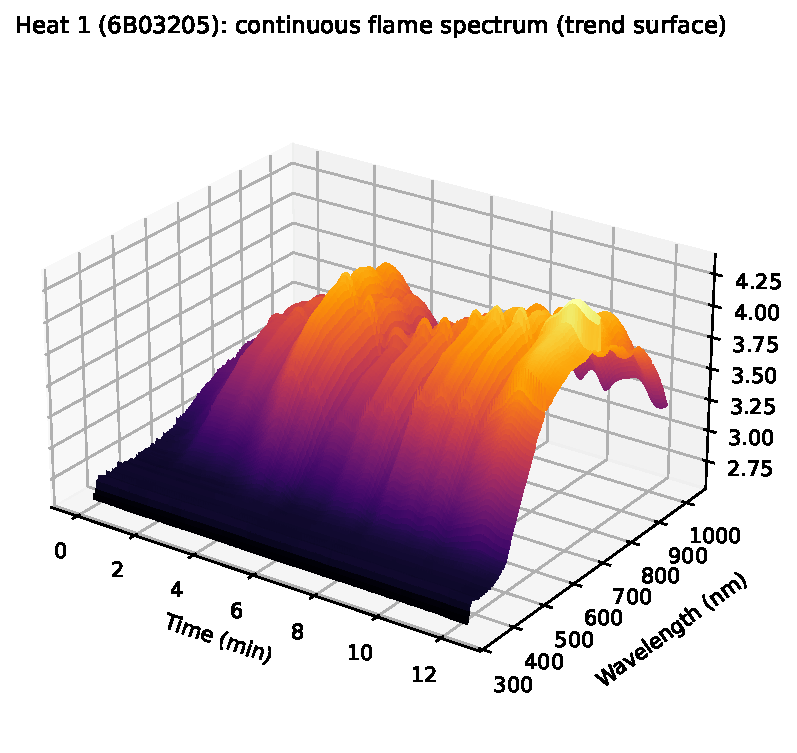
\includegraphics[width=.95\linewidth,height=.39\textheight,keepaspectratio]{figures/q1_surface_heat01.pdf}
\caption{Continuous spectral trend surface for Heat 1.}
\end{figure}
\begin{figure}[!htbp]
\centering
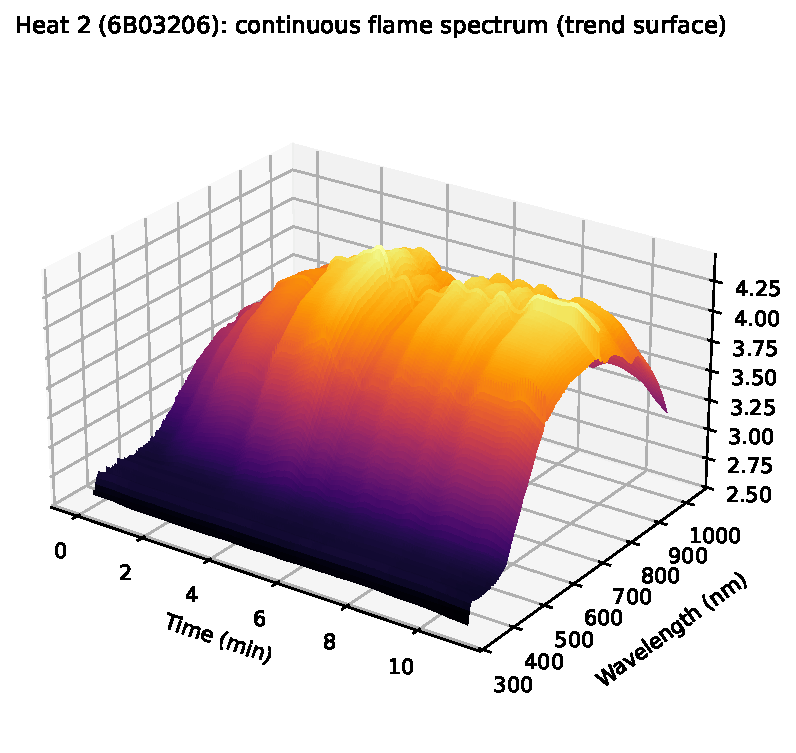
\includegraphics[width=.95\linewidth,height=.39\textheight,keepaspectratio]{figures/q1_surface_heat02.pdf}
\caption{Continuous spectral trend surface for Heat 2.}
\end{figure}
\begin{figure}[!htbp]
\centering
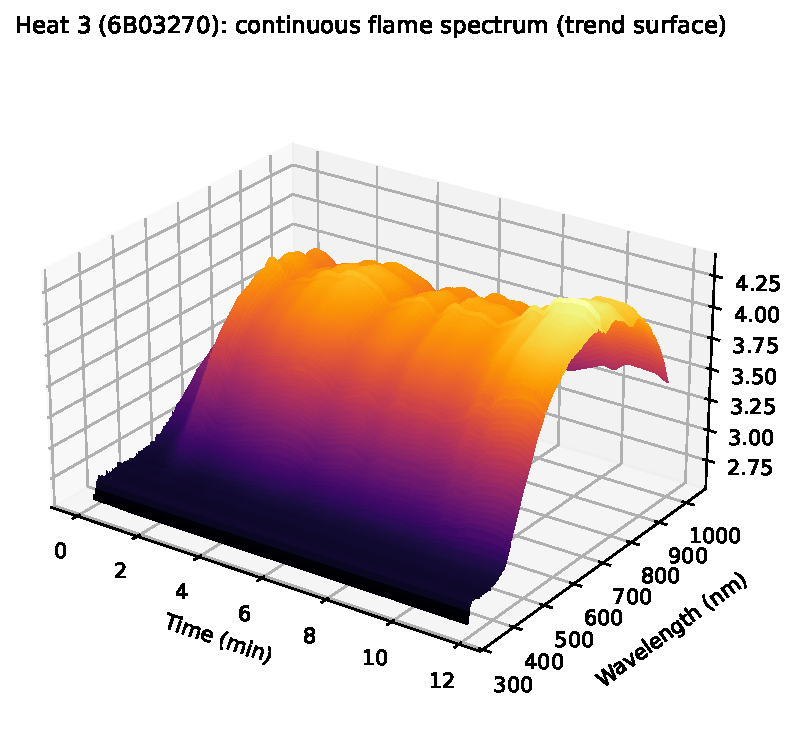
\includegraphics[width=.95\linewidth,height=.39\textheight,keepaspectratio]{figures/q1_surface_heat03.pdf}
\caption{Continuous spectral trend surface for Heat 3.}
\end{figure}
\begin{figure}[!htbp]
\centering
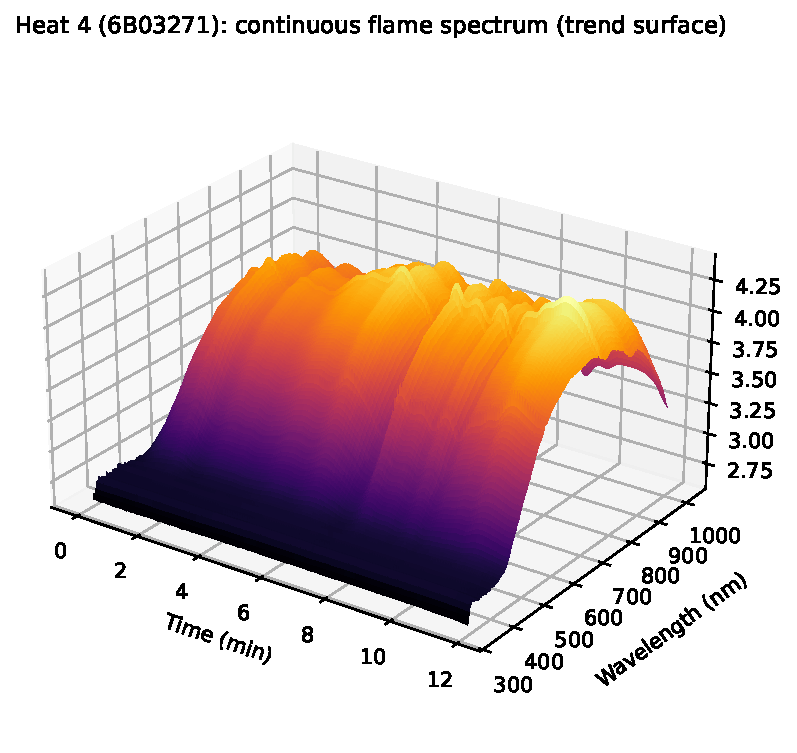
\includegraphics[width=.95\linewidth,height=.39\textheight,keepaspectratio]{figures/q1_surface_heat04.pdf}
\caption{Continuous spectral trend surface for Heat 4.}
\end{figure}
\begin{figure}[!htbp]
\centering
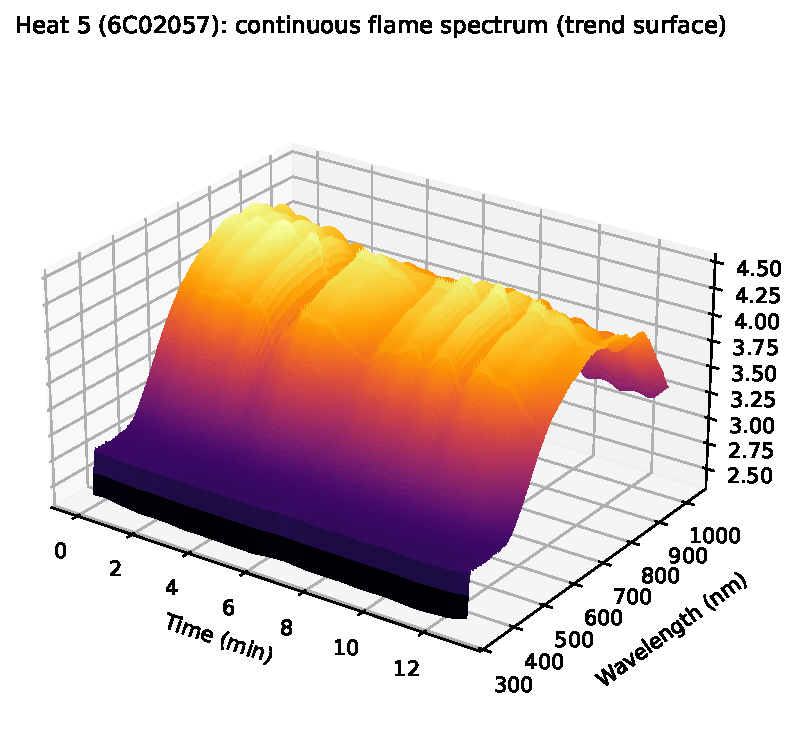
\includegraphics[width=.95\linewidth,height=.39\textheight,keepaspectratio]{figures/q1_surface_heat05.pdf}
\caption{Continuous spectral trend surface for Heat 5.}
\end{figure}
\begin{figure}[!htbp]
\centering
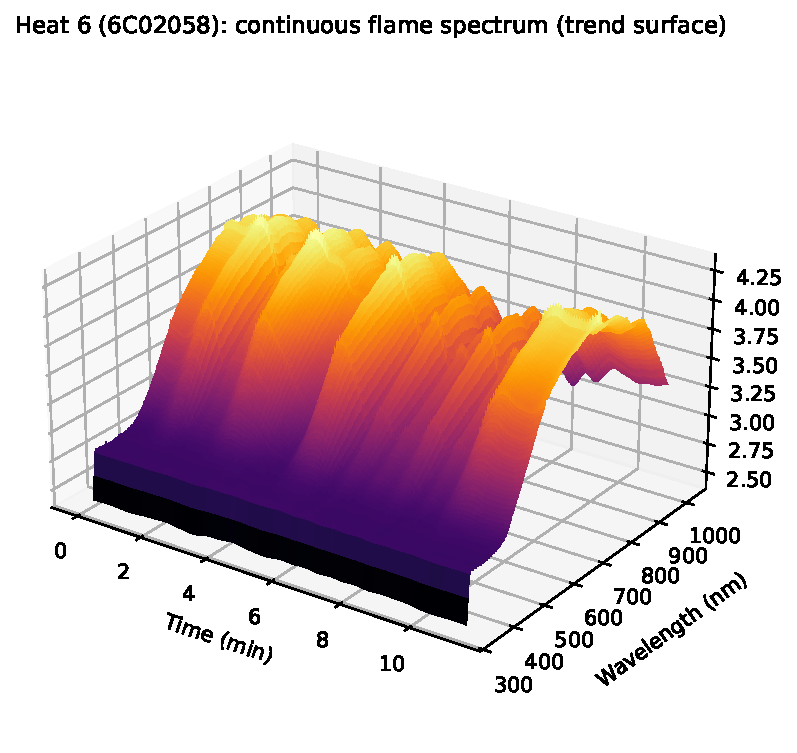
\includegraphics[width=.95\linewidth,height=.39\textheight,keepaspectratio]{figures/q1_surface_heat06.pdf}
\caption{Continuous spectral trend surface for Heat 6.}
\end{figure}
\begin{figure}[!htbp]
\centering
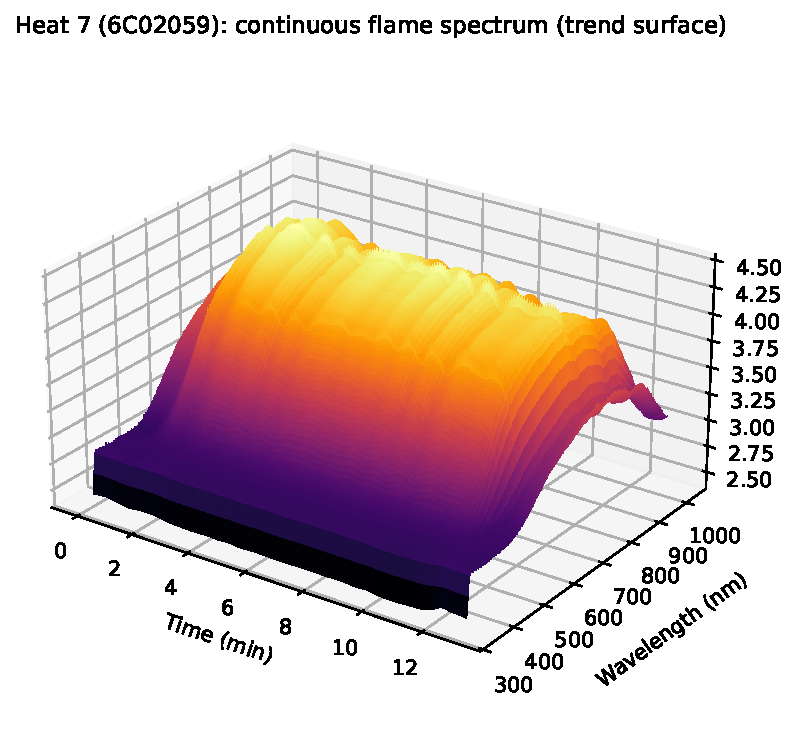
\includegraphics[width=.95\linewidth,height=.39\textheight,keepaspectratio]{figures/q1_surface_heat07.pdf}
\caption{Continuous spectral trend surface for Heat 7.}
\end{figure}
\begin{figure}[!htbp]
\centering
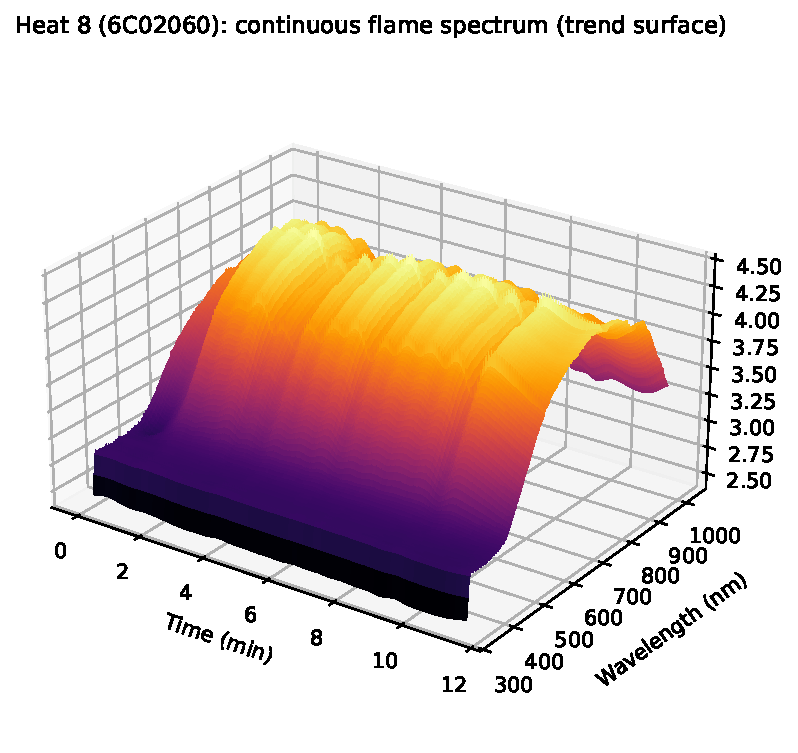
\includegraphics[width=.95\linewidth,height=.39\textheight,keepaspectratio]{figures/q1_surface_heat08.pdf}
\caption{Continuous spectral trend surface for Heat 8.}
\end{figure}
\begin{figure}[!htbp]
\centering
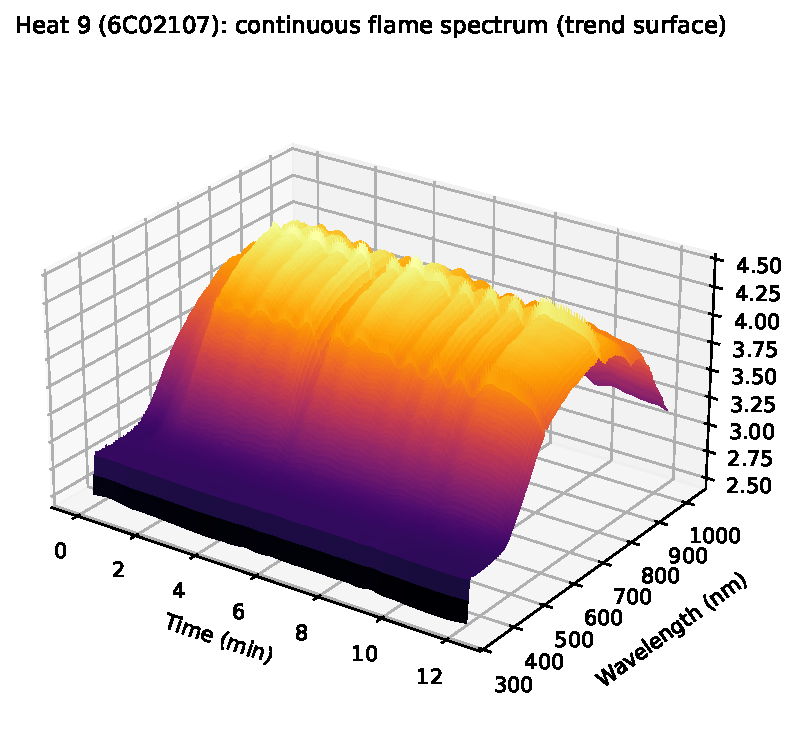
\includegraphics[width=.95\linewidth,height=.39\textheight,keepaspectratio]{figures/q1_surface_heat09.pdf}
\caption{Continuous spectral trend surface for Heat 9.}
\end{figure}
\begin{figure}[!htbp]
\centering
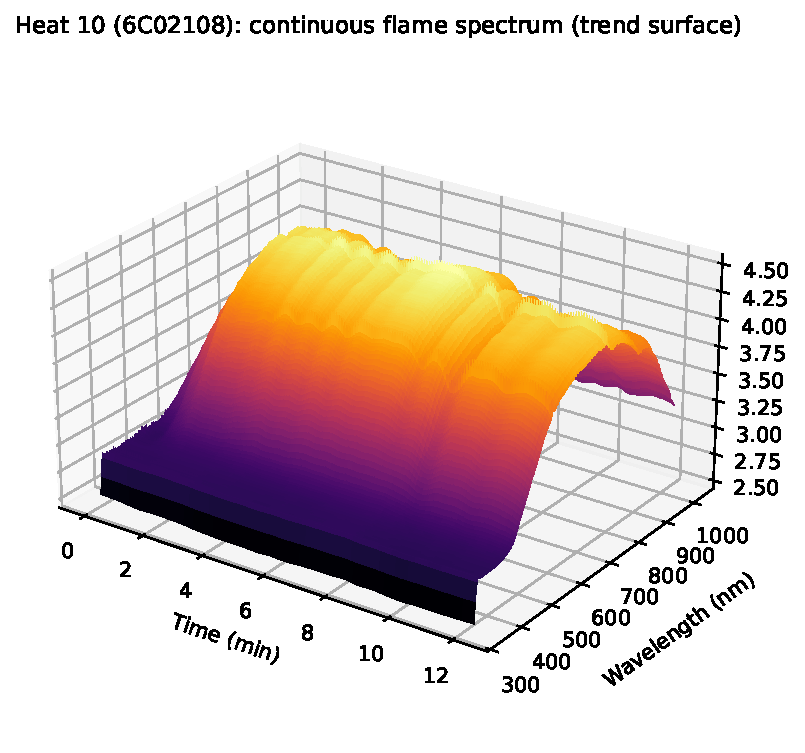
\includegraphics[width=.95\linewidth,height=.39\textheight,keepaspectratio]{figures/q1_surface_heat10.pdf}
\caption{Continuous spectral trend surface for Heat 10.}
\end{figure}
\FloatBarrier
\subsection{Process Curves}
\begin{figure}[!htbp]
\centering
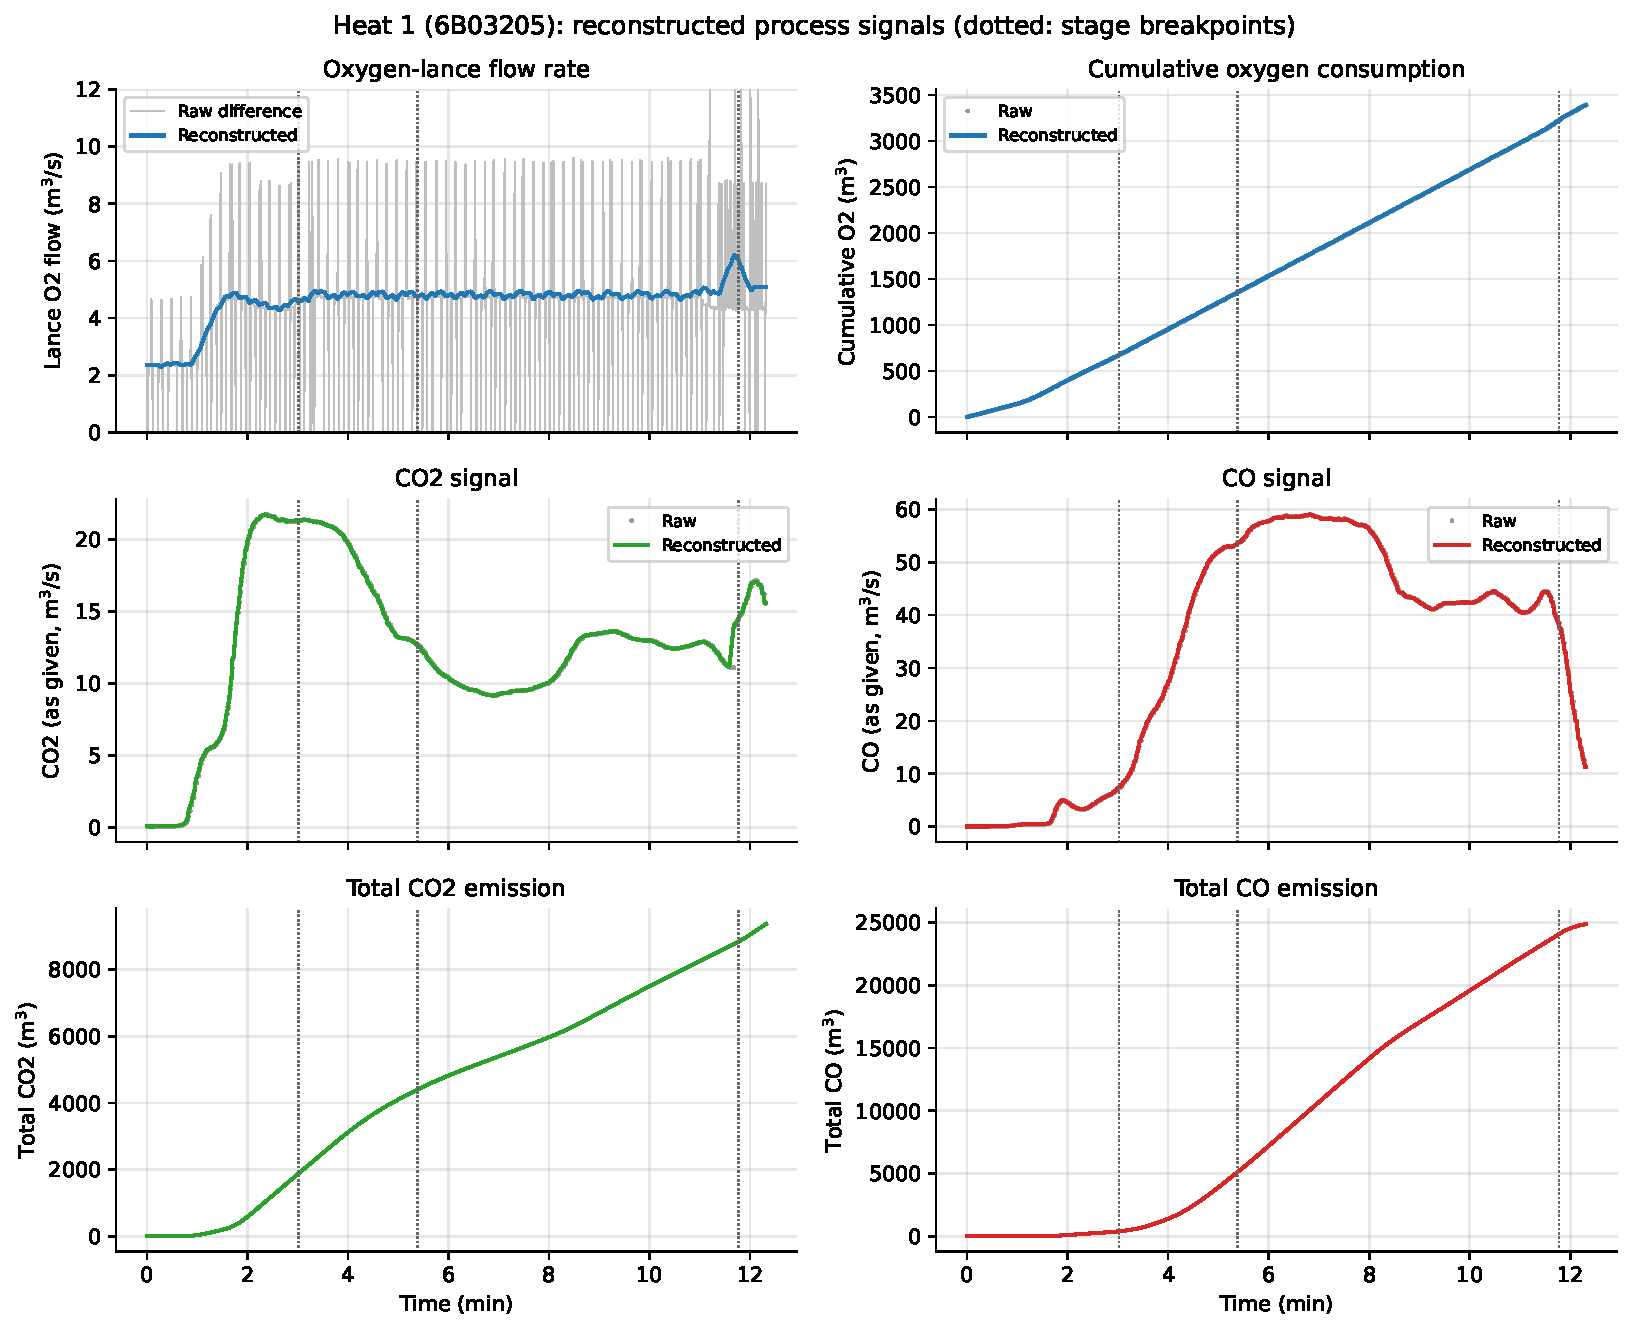
\includegraphics[width=.95\linewidth,height=.39\textheight,keepaspectratio]{figures/q2_curves_heat01.pdf}
\caption{Reconstructed process curves for Heat 1.}
\end{figure}
\begin{figure}[!htbp]
\centering
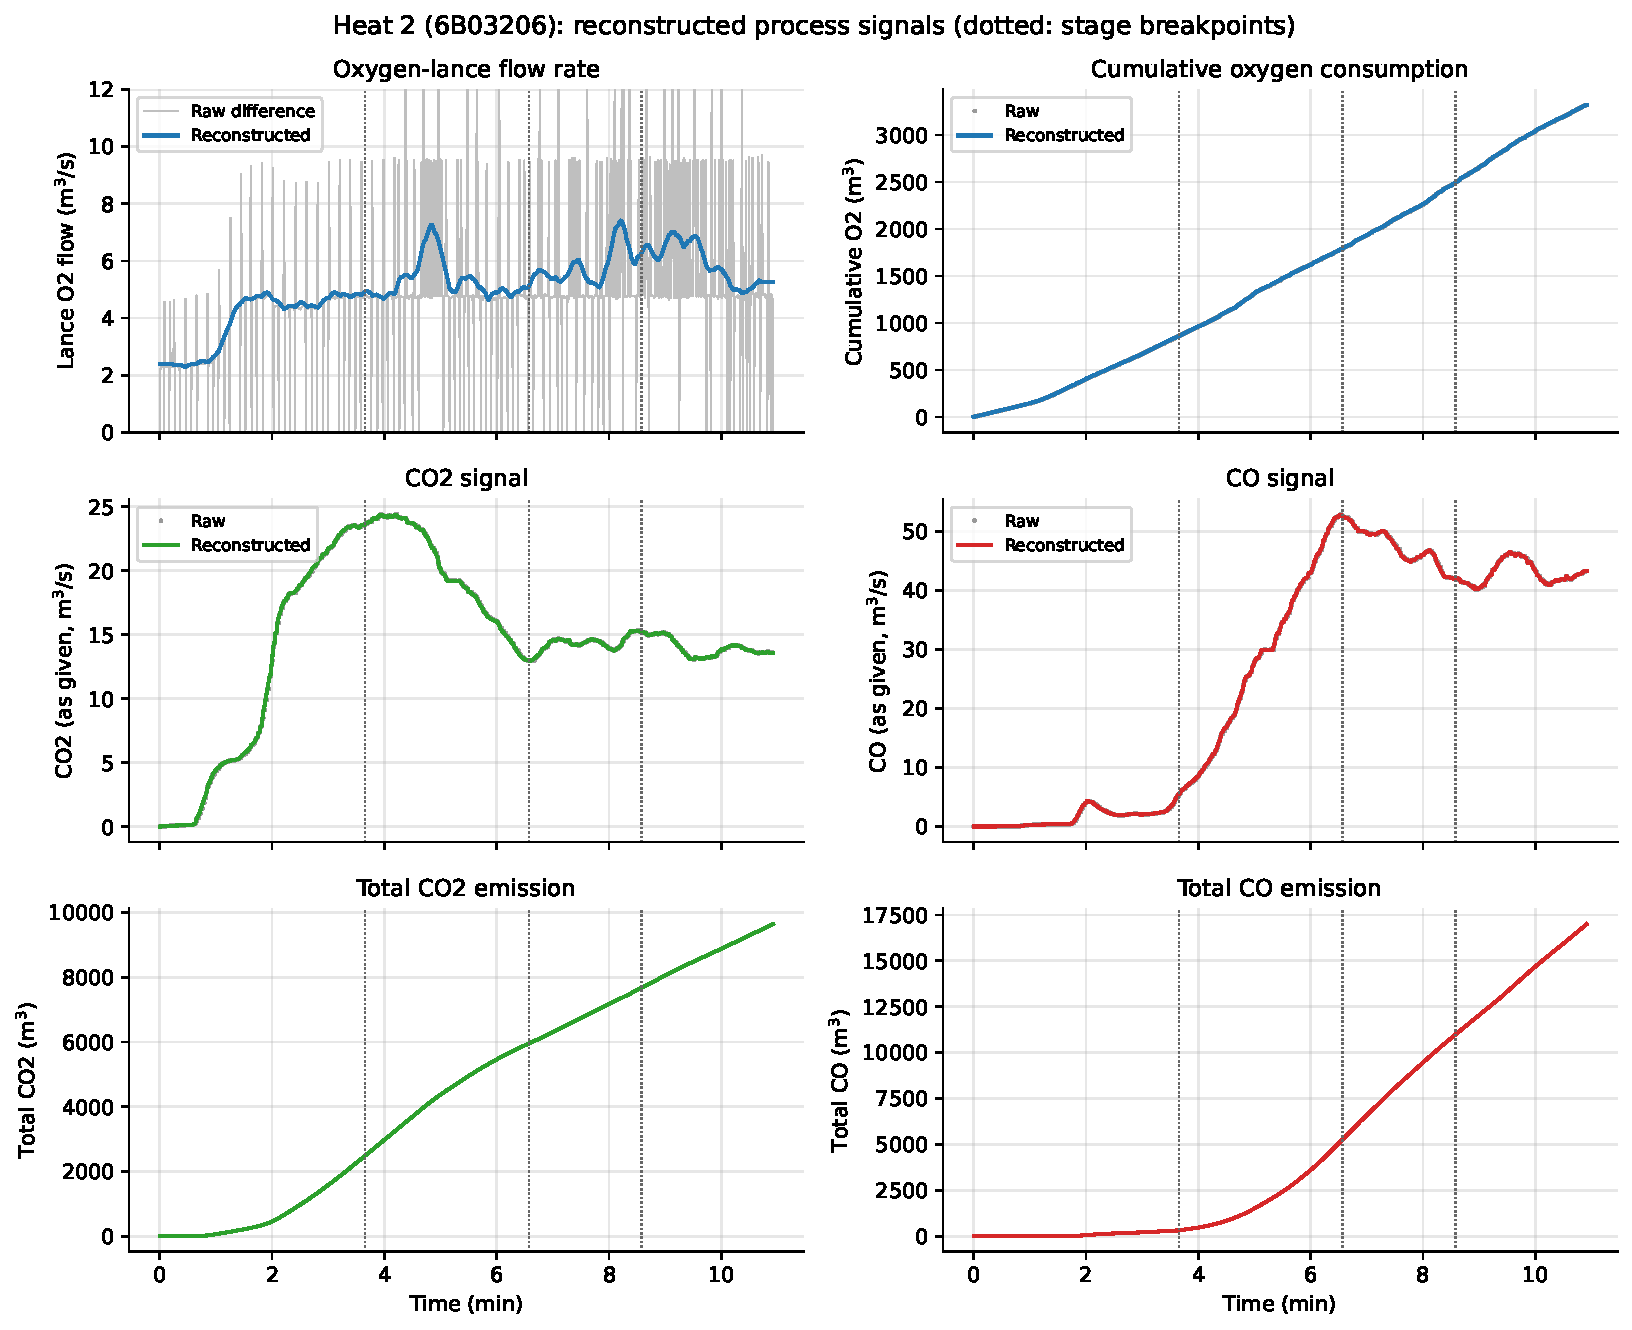
\includegraphics[width=.95\linewidth,height=.39\textheight,keepaspectratio]{figures/q2_curves_heat02.pdf}
\caption{Reconstructed process curves for Heat 2.}
\end{figure}
\begin{figure}[!htbp]
\centering
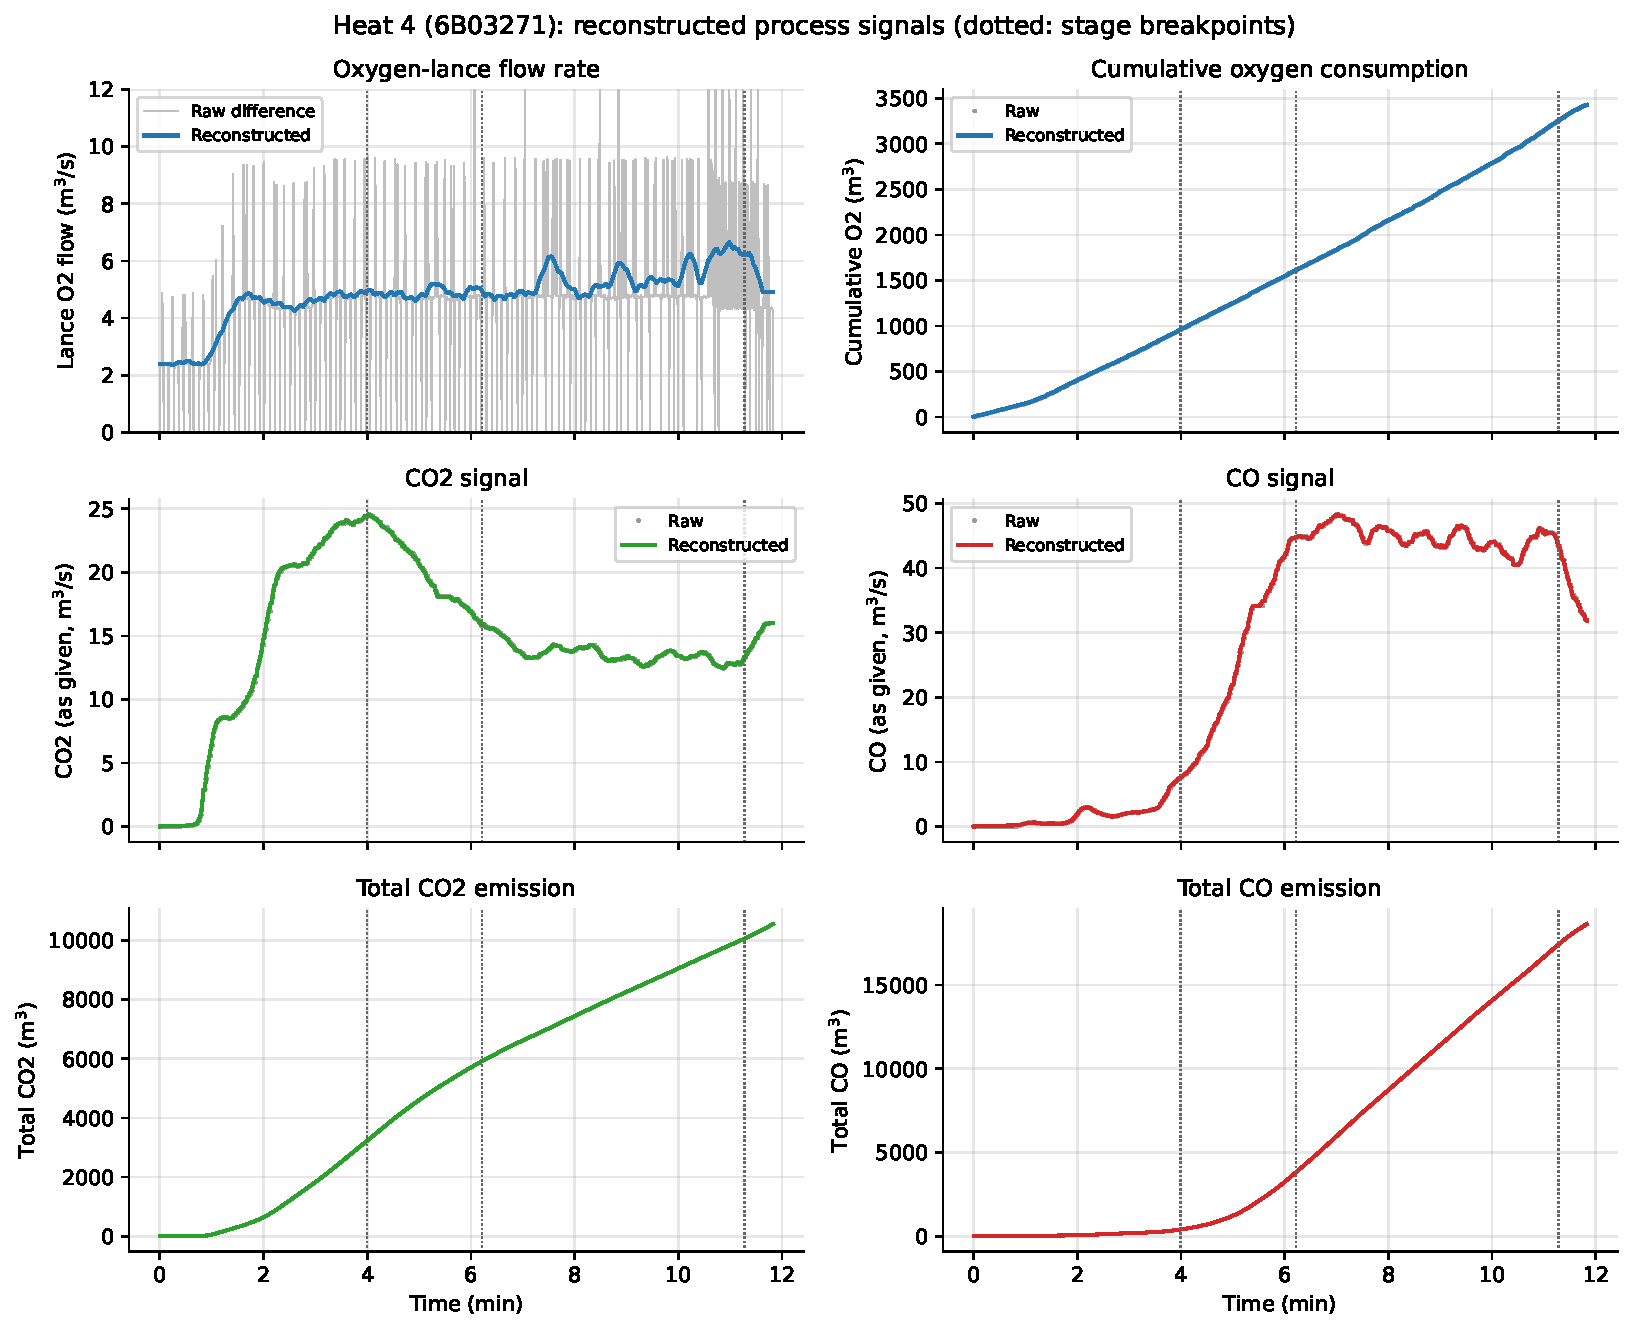
\includegraphics[width=.95\linewidth,height=.39\textheight,keepaspectratio]{figures/q2_curves_heat04.pdf}
\caption{Reconstructed process curves for Heat 4.}
\end{figure}
\begin{figure}[!htbp]
\centering
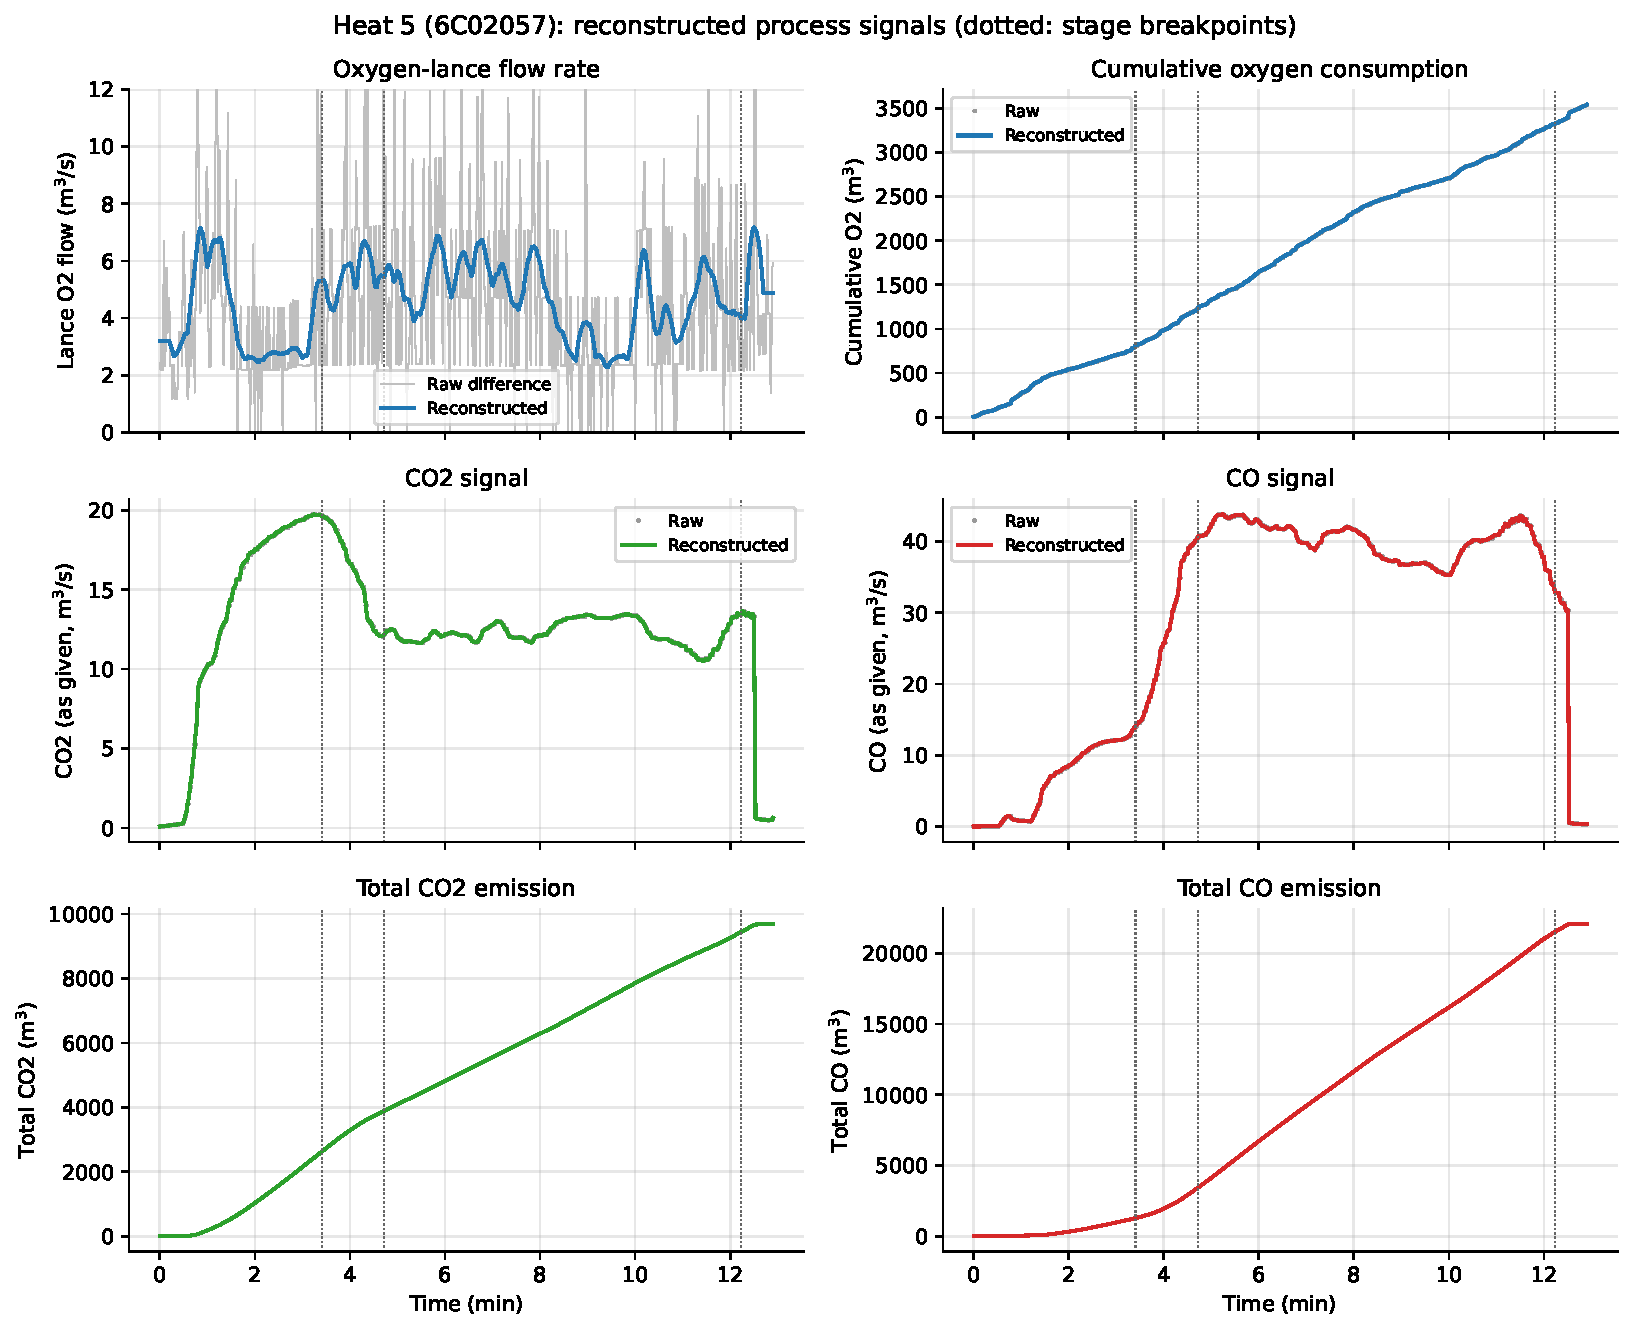
\includegraphics[width=.95\linewidth,height=.39\textheight,keepaspectratio]{figures/q2_curves_heat05.pdf}
\caption{Reconstructed process curves for Heat 5.}
\end{figure}
\begin{figure}[!htbp]
\centering
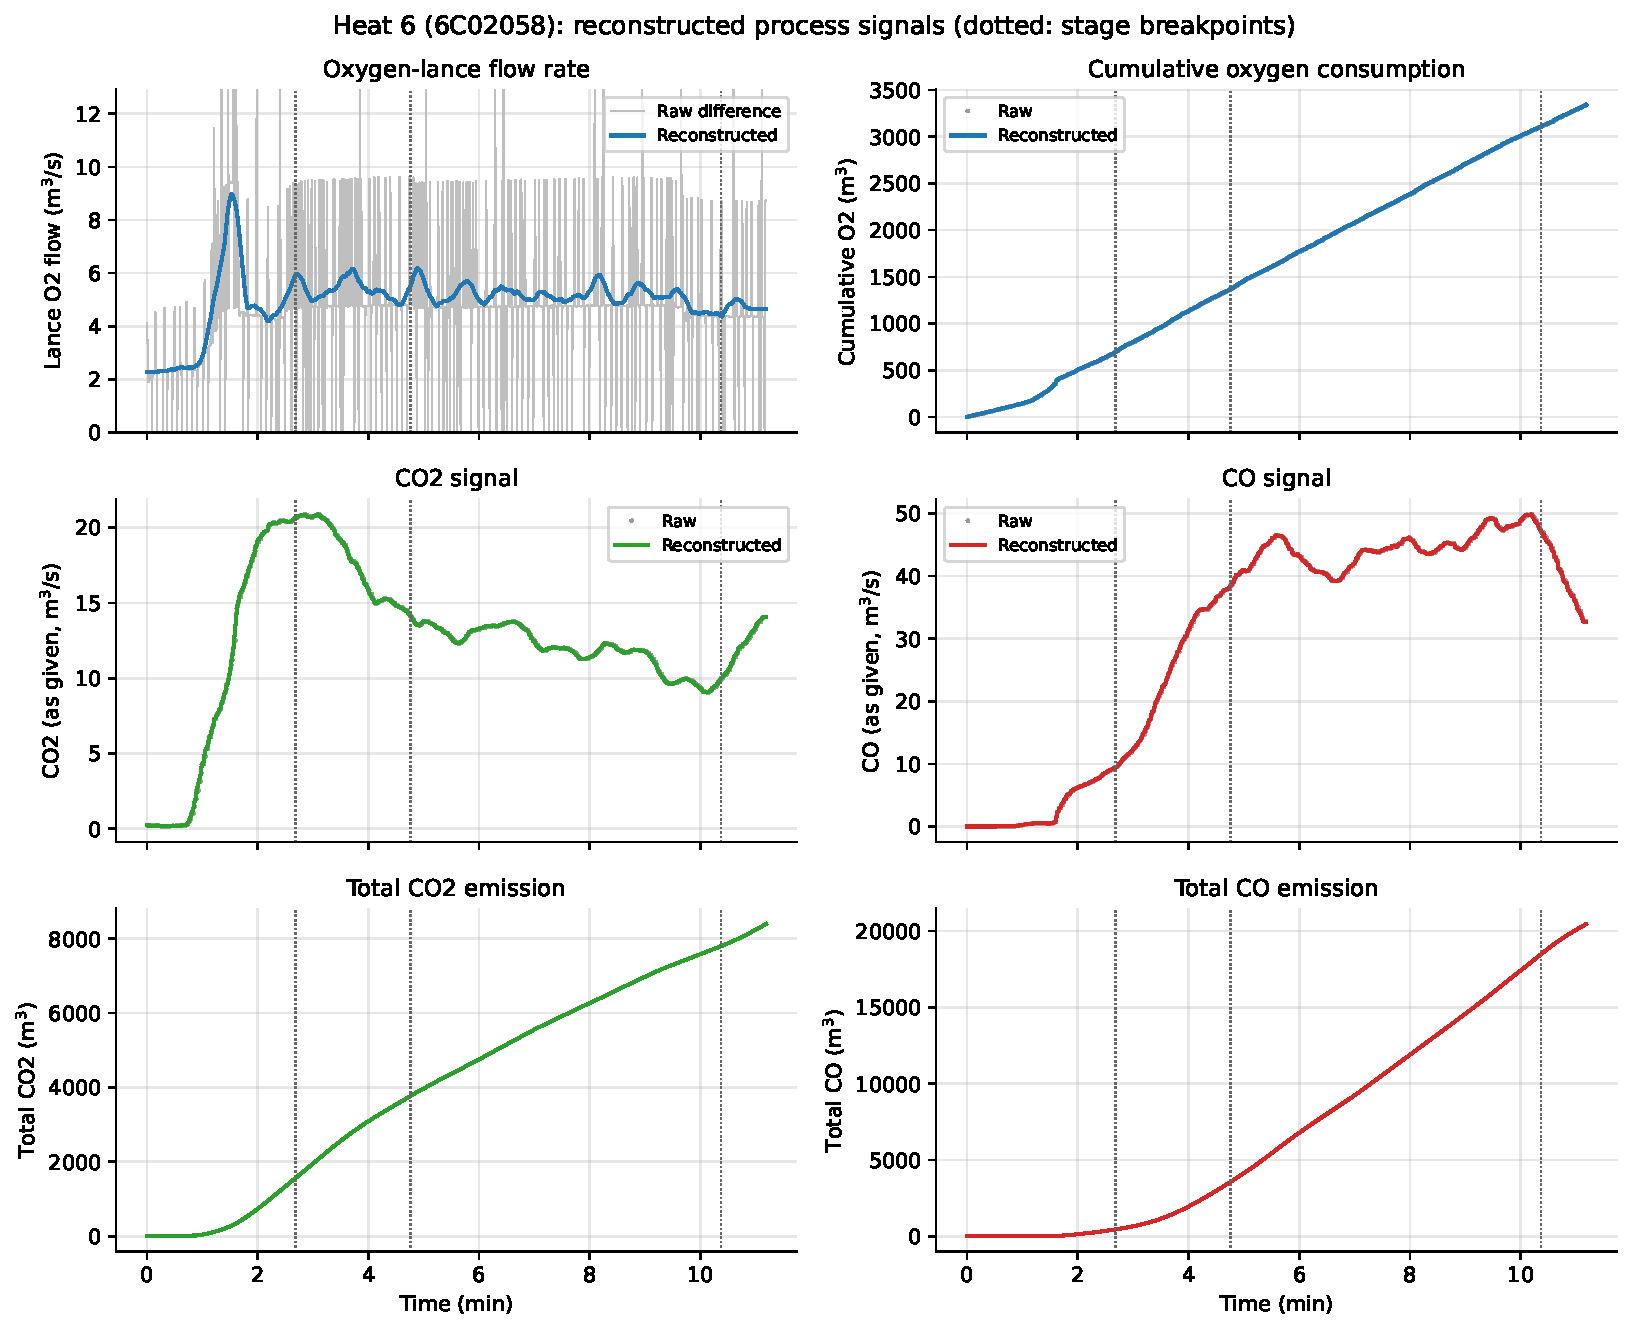
\includegraphics[width=.95\linewidth,height=.39\textheight,keepaspectratio]{figures/q2_curves_heat06.pdf}
\caption{Reconstructed process curves for Heat 6.}
\end{figure}
\begin{figure}[!htbp]
\centering
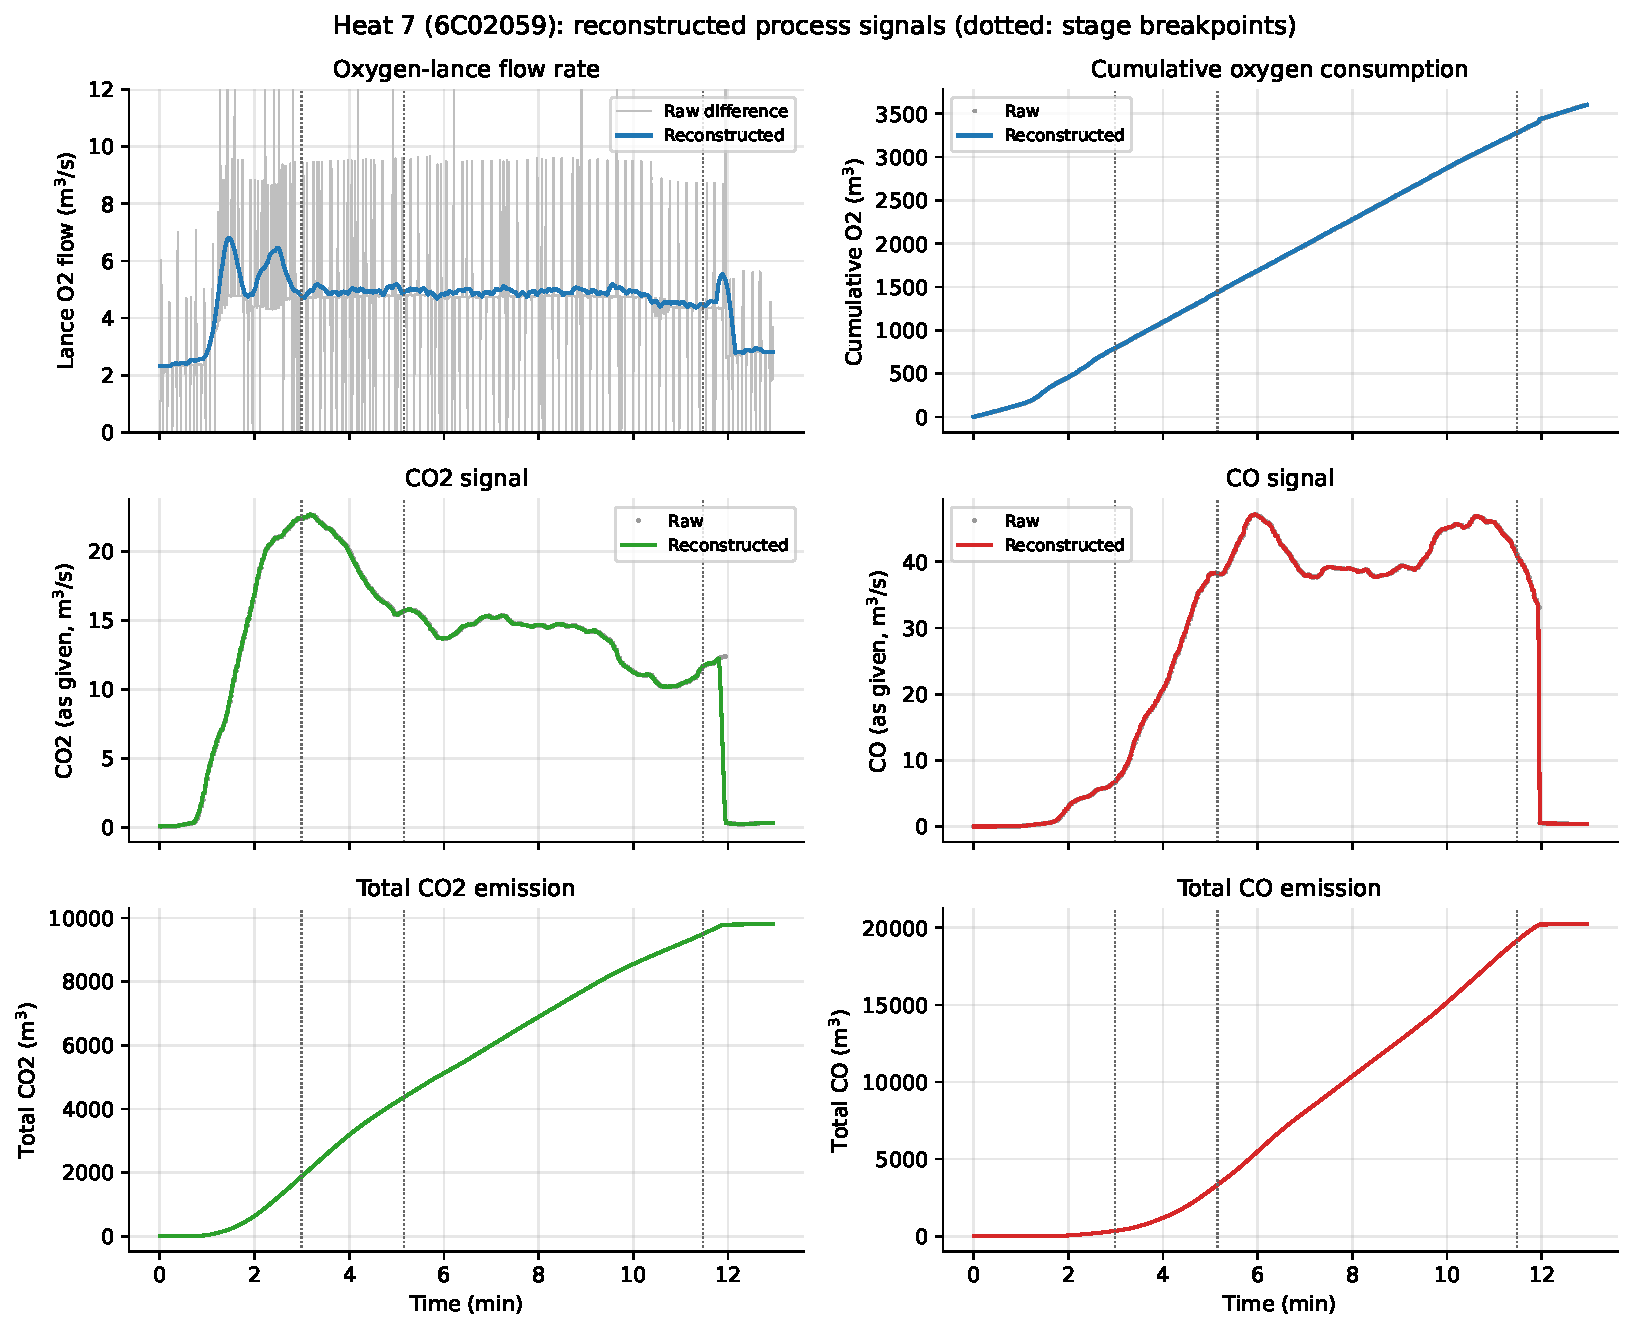
\includegraphics[width=.95\linewidth,height=.39\textheight,keepaspectratio]{figures/q2_curves_heat07.pdf}
\caption{Reconstructed process curves for Heat 7.}
\end{figure}
\begin{figure}[!htbp]
\centering
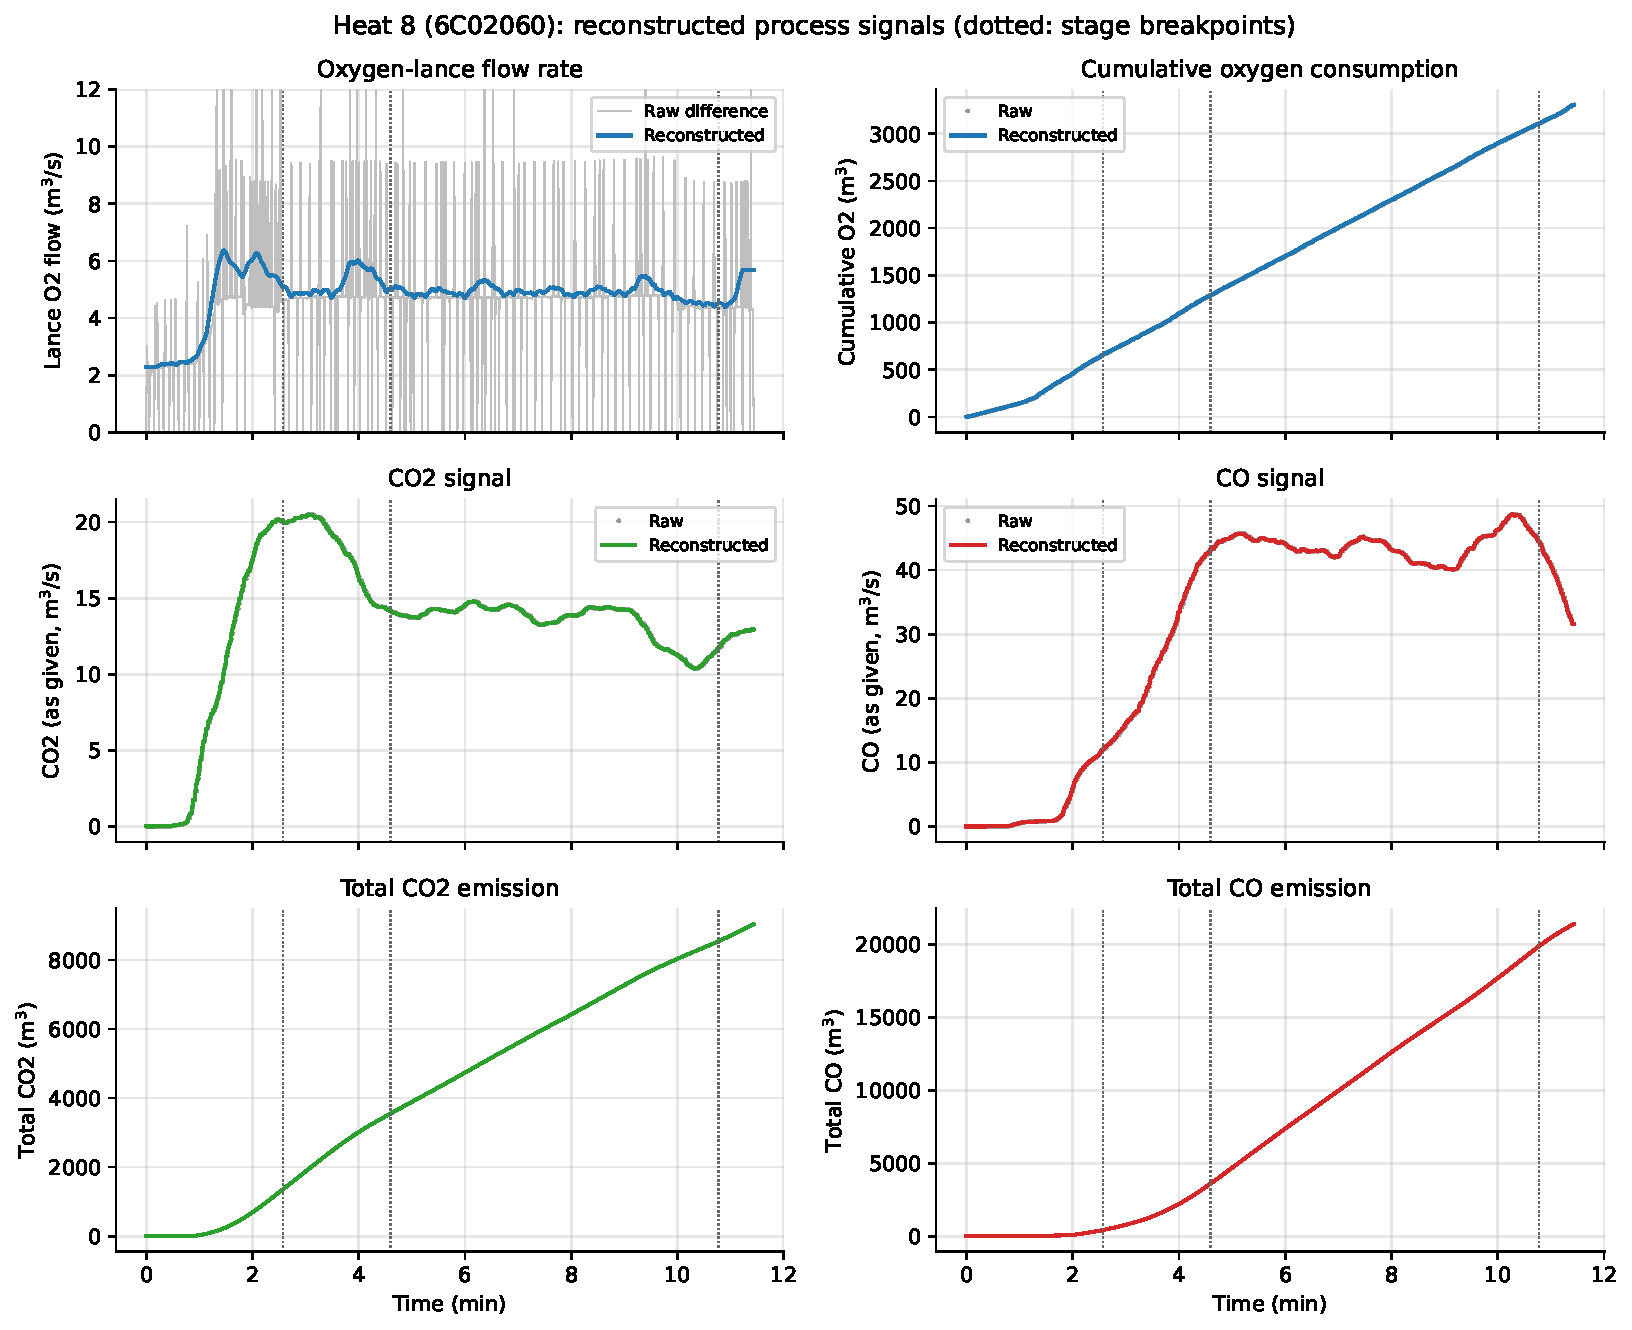
\includegraphics[width=.95\linewidth,height=.39\textheight,keepaspectratio]{figures/q2_curves_heat08.pdf}
\caption{Reconstructed process curves for Heat 8.}
\end{figure}
\begin{figure}[!htbp]
\centering
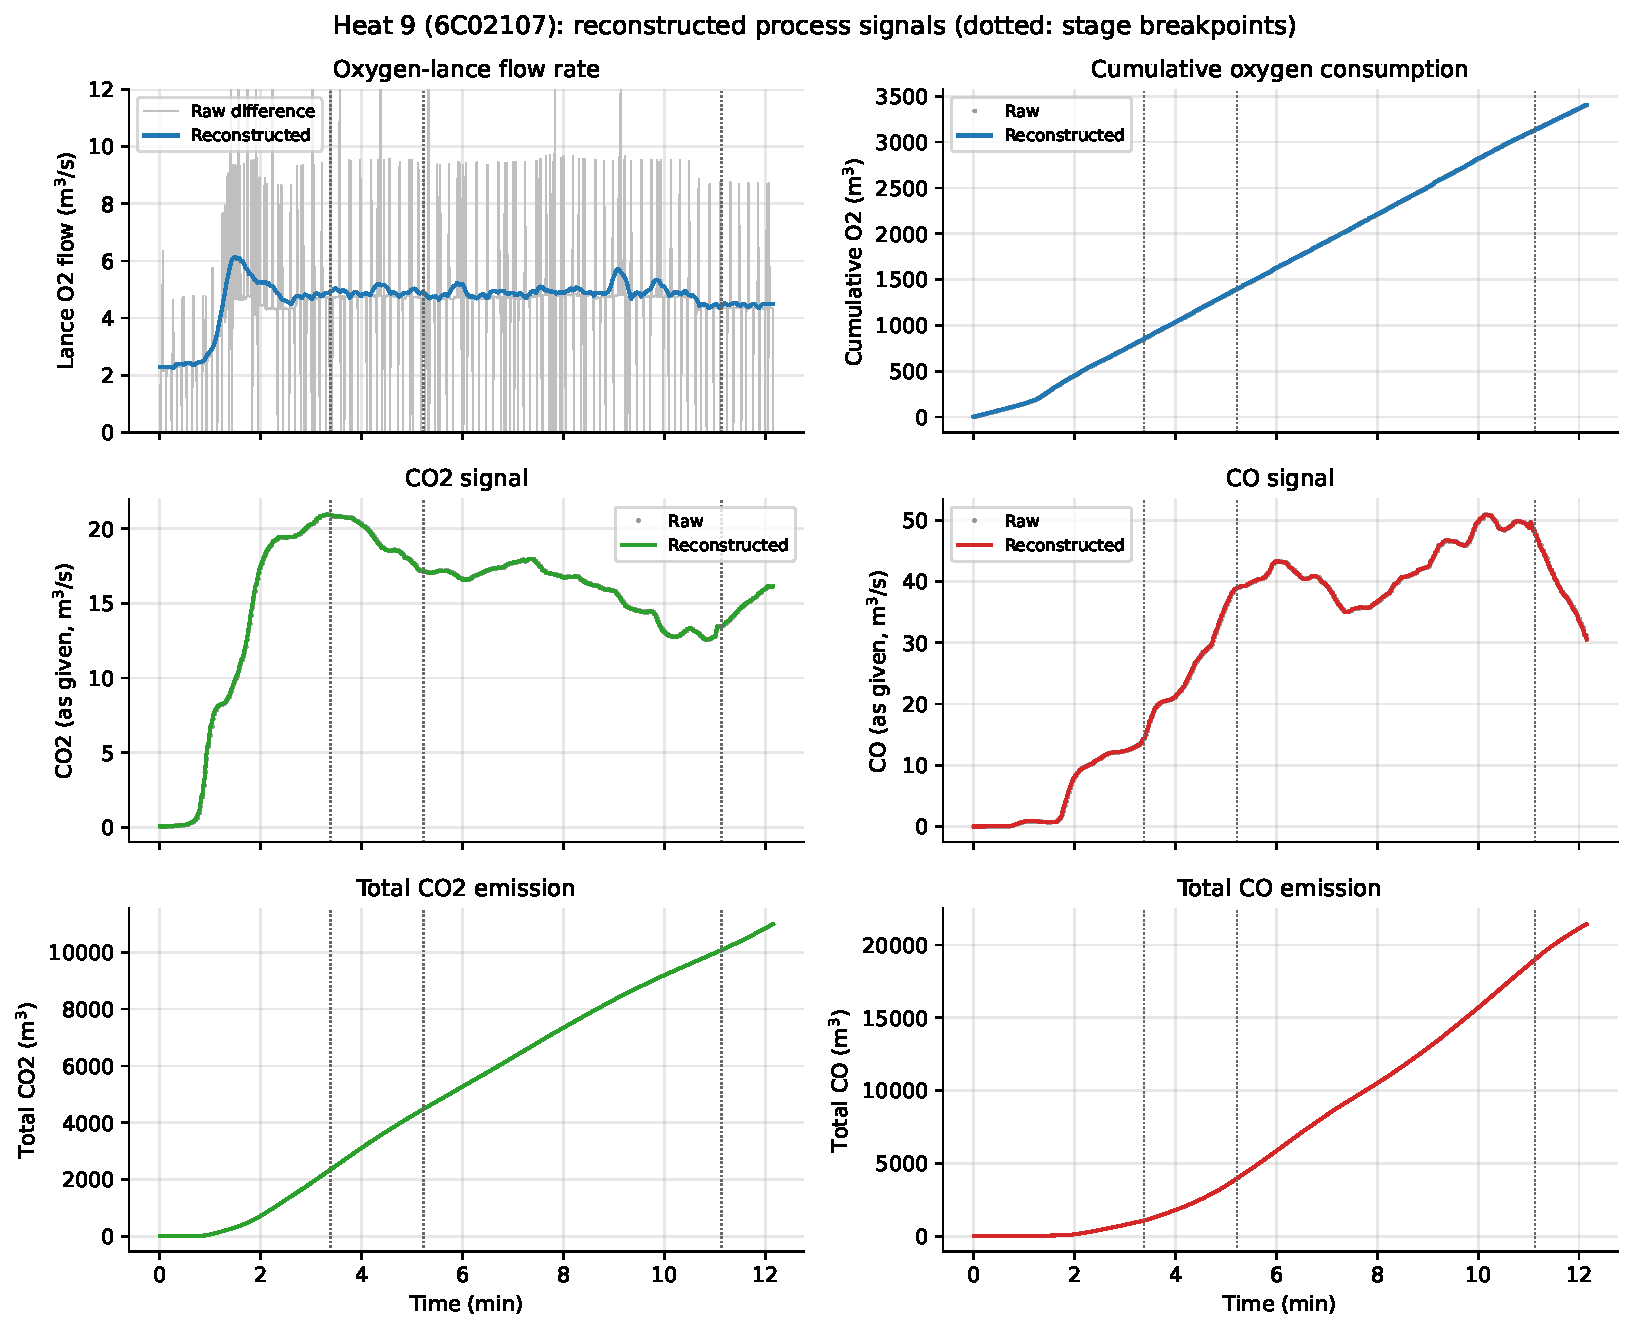
\includegraphics[width=.95\linewidth,height=.39\textheight,keepaspectratio]{figures/q2_curves_heat09.pdf}
\caption{Reconstructed process curves for Heat 9.}
\end{figure}
\begin{figure}[!htbp]
\centering
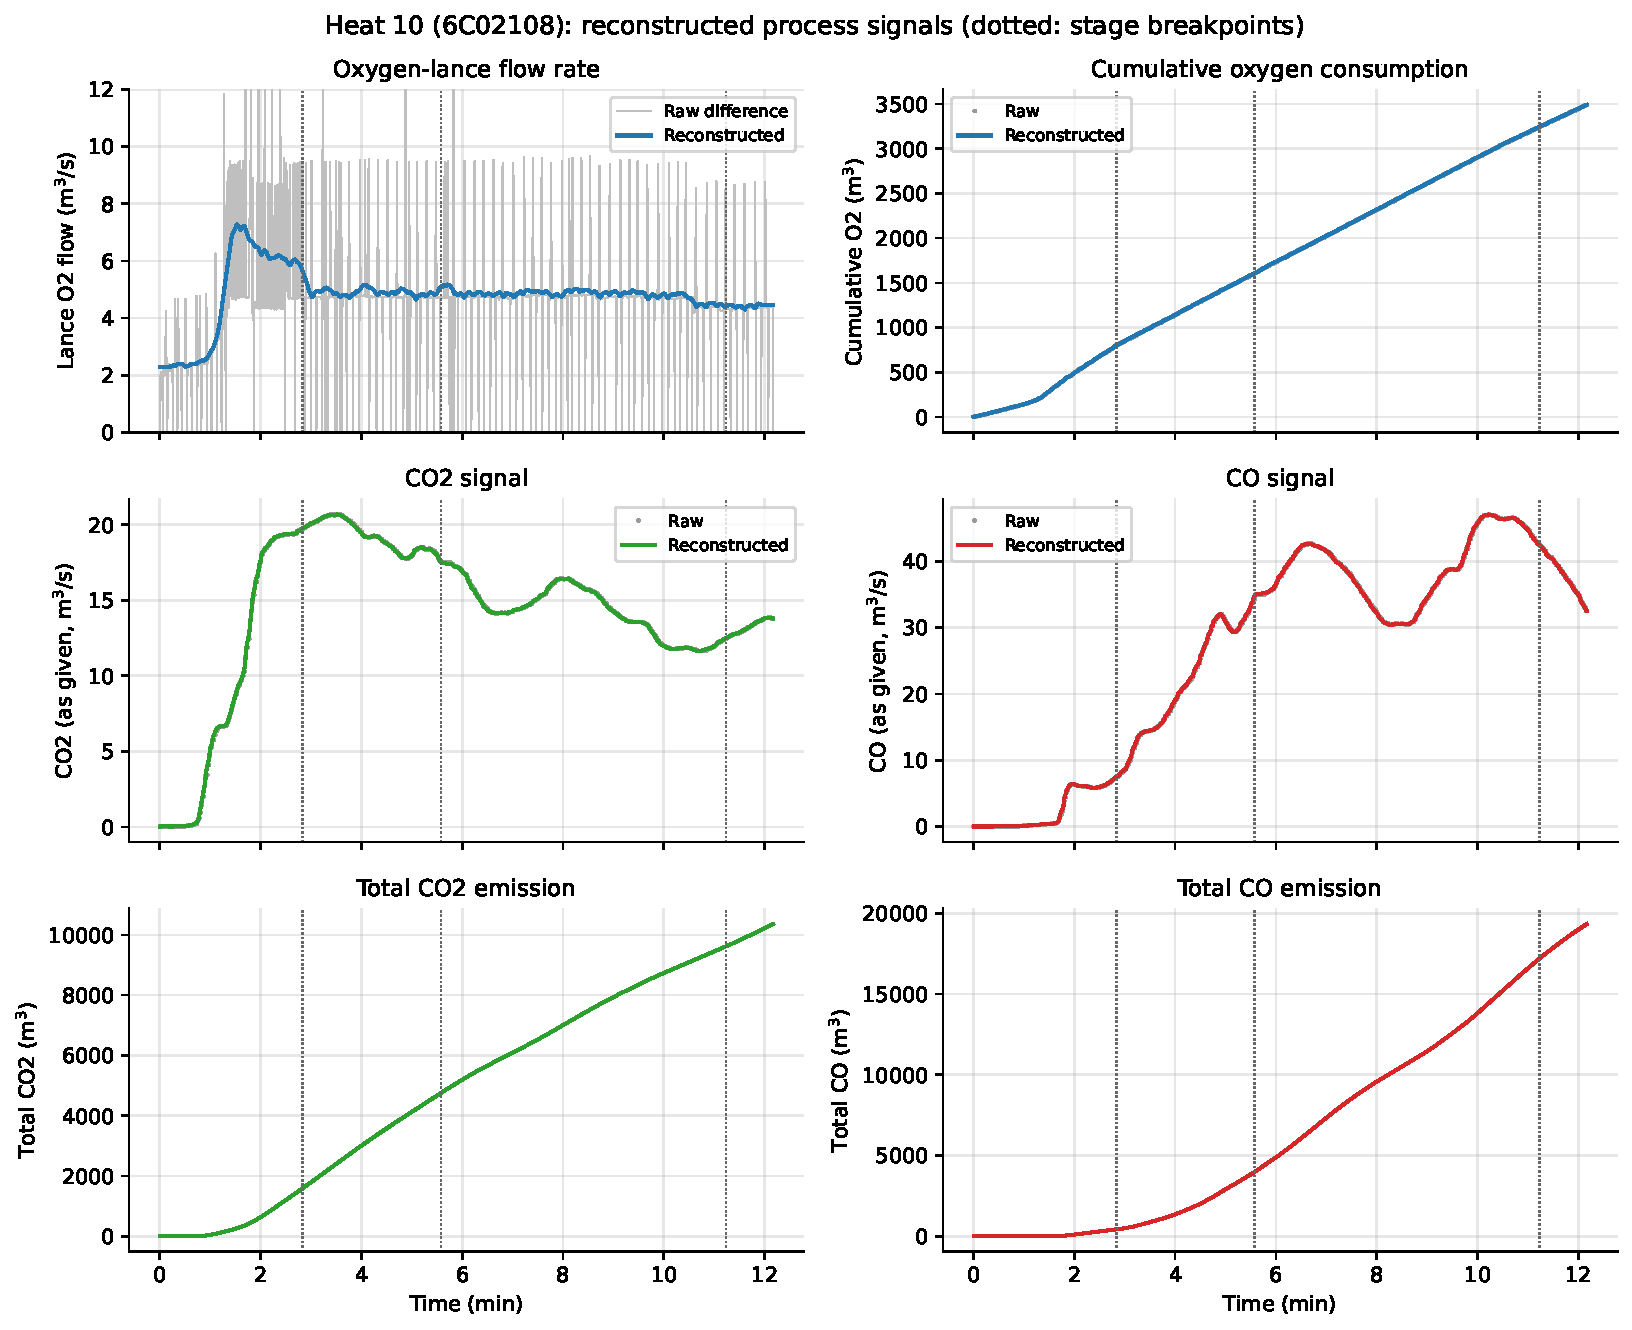
\includegraphics[width=.95\linewidth,height=.39\textheight,keepaspectratio]{figures/q2_curves_heat10.pdf}
\caption{Reconstructed process curves for Heat 10.}
\end{figure}
\FloatBarrier
\clearpage
\section{Software and Source Code}\label{app:code}
Software: Python 3.13, NumPy, SciPy, pandas, scikit-learn, XGBoost, LightGBM, Matplotlib, and python-calamine. The code is listed in execution-package groups. Non-ASCII characters in the source listing are displayed as Unicode escapes.

\subsection{Spectral reconstruction and supporting analyses}
\subsubsection*{\texttt{common.py}}
\VerbatimInput[fontsize=\scriptsize,breaklines,breakanywhere,breakanywheresymbolpre={},numbers=left,numbersep=4pt]{source-listings/task1-common.py}
\subsubsection*{\texttt{fig\_q2\_o2\_beat.py}}
\VerbatimInput[fontsize=\scriptsize,breaklines,breakanywhere,breakanywheresymbolpre={},numbers=left,numbersep=4pt]{source-listings/task1-fig_q2_o2_beat.py}
\subsubsection*{\texttt{q0\_prepare.py}}
\VerbatimInput[fontsize=\scriptsize,breaklines,breakanywhere,breakanywheresymbolpre={},numbers=left,numbersep=4pt]{source-listings/task1-q0_prepare.py}
\subsubsection*{\texttt{q1\_spectra.py}}
\VerbatimInput[fontsize=\scriptsize,breaklines,breakanywhere,breakanywheresymbolpre={},numbers=left,numbersep=4pt]{source-listings/task1-q1_spectra.py}
\subsubsection*{\texttt{q2a\_process.py}}
\VerbatimInput[fontsize=\scriptsize,breaklines,breakanywhere,breakanywheresymbolpre={},numbers=left,numbersep=4pt]{source-listings/task1-q2a_process.py}
\subsubsection*{\texttt{q2b\_delay.py}}
\VerbatimInput[fontsize=\scriptsize,breaklines,breakanywhere,breakanywheresymbolpre={},numbers=left,numbersep=4pt]{source-listings/task1-q2b_delay.py}
\subsubsection*{\texttt{q3\_predict.py}}
\VerbatimInput[fontsize=\scriptsize,breaklines,breakanywhere,breakanywheresymbolpre={},numbers=left,numbersep=4pt]{source-listings/task1-q3_predict.py}
\subsubsection*{\texttt{run\_all.sh}}
\VerbatimInput[fontsize=\scriptsize,breaklines,breakanywhere,breakanywheresymbolpre={},numbers=left,numbersep=4pt]{source-listings/task1-run_all.sh}
\subsubsection*{\texttt{sens\_delay\_misestimation.py}}
\VerbatimInput[fontsize=\scriptsize,breaklines,breakanywhere,breakanywheresymbolpre={},numbers=left,numbersep=4pt]{source-listings/task1-sens_delay_misestimation.py}
\subsection{Delay model and cross-heat prediction}
\subsubsection*{\texttt{config.py}}
\VerbatimInput[fontsize=\scriptsize,breaklines,breakanywhere,breakanywheresymbolpre={},numbers=left,numbersep=4pt]{source-listings/task23-config.py}
\subsubsection*{\texttt{io\_loader.py}}
\VerbatimInput[fontsize=\scriptsize,breaklines,breakanywhere,breakanywheresymbolpre={},numbers=left,numbersep=4pt]{source-listings/task23-io_loader.py}
\subsubsection*{\texttt{main.py}}
\VerbatimInput[fontsize=\scriptsize,breaklines,breakanywhere,breakanywheresymbolpre={},numbers=left,numbersep=4pt]{source-listings/task23-main.py}
\subsubsection*{\texttt{q1\_spectral\_recon.py}}
\VerbatimInput[fontsize=\scriptsize,breaklines,breakanywhere,breakanywheresymbolpre={},numbers=left,numbersep=4pt]{source-listings/task23-q1_spectral_recon.py}
\subsubsection*{\texttt{q2\_gas\_delay.py}}
\VerbatimInput[fontsize=\scriptsize,breaklines,breakanywhere,breakanywheresymbolpre={},numbers=left,numbersep=4pt]{source-listings/task23-q2_gas_delay.py}
\subsubsection*{\texttt{q3\_fusion\_predict.py}}
\VerbatimInput[fontsize=\scriptsize,breaklines,breakanywhere,breakanywheresymbolpre={},numbers=left,numbersep=4pt]{source-listings/task23-q3_fusion_predict.py}
\subsubsection*{\texttt{scientific\_verify.py}}
\VerbatimInput[fontsize=\scriptsize,breaklines,breakanywhere,breakanywheresymbolpre={},numbers=left,numbersep=4pt]{source-listings/task23-scientific_verify.py}
